\documentclass[11pt,twocolumn,a4paper]{article}
\usepackage{amsmath}
\usepackage{amssymb}
\usepackage{graphicx}
\usepackage{booktabs}
\usepackage{hyperref}
\usepackage{float}
\usepackage{geometry}
\usepackage{xcolor}
\usepackage{microtype}
\usepackage{titlesec}
\usepackage{caption}
\usepackage{abstract}
\usepackage{fancyhdr}

% Page geometry matching Springer twocolumn style
\geometry{
    a4paper,
    left=15mm,
    right=15mm,
    top=22mm,
    bottom=22mm,
    footskip=10mm
}

\hypersetup{
    colorlinks=true,
    linkcolor=blue,
    filecolor=magenta,      
    urlcolor=cyan,
    pdftitle={Amelioration de l'evaluation du geopatrimoine au Maroc : un modele national d'accessibilite des geosites base sur l'aide a la decision spatiale multicritere floue (Fuzzy MCDSS) sous validation croisee par blocs spatiaux},
    pdfpagemode=FullScreen,
}

\raggedbottom

% Set up headers and footers to resemble the journal page
\pagestyle{fancy}
\fancyhf{}
\fancyhead[L]{\textsf{GSMI-UM6P}}
\fancyhead[R]{\textsf{Rapport Technique de Stage — Modèle Fuzzy MCDSS}}
\fancyfoot[C]{\thepage}
\renewcommand{\headrulewidth}{0.4pt}
\renewcommand{\footrulewidth}{0pt}

% Section formatting matching Springer
\titleformat{\section}{\large\bfseries\sffamily}{\thesection}{1em}{}
\titleformat{\subsection}{\normalsize\bfseries\sffamily}{\thesubsection}{1em}{}

% Redefine abstract style
\renewenvironment{abstract}{%
    \small\sffamily
    \noindent\textbf{Résumé}\quad
    \selectfont
}{%
    \vspace{0.4cm}
}

\begin{document}

% GSMI Header on first page
\twocolumn[
    \begin{@twocolumnfalse}
        \begin{center}
            {
\includegraphics[width=0.45\textwidth]{../um6p_figures/um6p_gsmi_logo.png}}
        \end{center}
        \vspace{0.4cm}
        
        {\Huge\bfseries\sffamily Amélioration de l'évaluation du géopatrimoine au Maroc : un modèle national d'accessibilité des géosites basé sur l'aide à la décision spatiale multicritère floue (Fuzzy MCDSS) et l'apprentissage automatique sous validation croisée par blocs spatiaux\par}
        \vspace{0.6cm}
        
        {\large\textbf{EL GORRIM Mohamed}\par}
        {\small\sffamily Stagiaire de recherche en IA, Geology and Sustainable Mining Institute (GSMI), Université Mohammed VI Polytechnique (UM6P), Ben Guerir, Maroc\par}
        \vspace{0.4cm}
        {\small\sffamily\textbf{Préparé pour :} Dr. Ismail BEN AMAR, Sanae EL HARCHE et Mohamed EL OUALI\par}
        \vspace{0.6cm}
        
        \begin{abstract}
        L'évaluation de l'accessibilité des sites du patrimoine géologique (géosites) sur de vastes territoires est essentielle pour la planification du géotourisme durable et de la conservation. S'appuyant sur le cadre d'apprentissage automatique (ML) localisé établi par Naimi et al. (2025) pour le bassin versant supérieur du Ziz, ce travail présente une mise à l'échelle nationale de la modélisation des géosites à l'ensemble du territoire marocain, en intégrant la proximité des infrastructures de transport réelles d'OpenStreetMap (OSM) et un moteur d'Aide à la Décision Spatiale Multicritère Floue (Fuzzy MCDSS). Nous compilons et standardisons une base de données de coordonnées de 375 géosites et extrayons les réseaux de transport nationaux depuis OSM pour calculer les distances exactes aux routes majeures (autoroutes et routes nationales) et aux pistes. En intégrant ces distances avec 6 caractéristiques physiques et routières clés de système d'information géographique (SIG) sous la projection Sahara Lambert (EPSG:26191), nous mettons en œuvre un modèle de décision hiérarchique flou guidé par des experts pour classer les géosites en trois catégories d'accessibilité : Facile, Modérée et Difficile. Pour traiter le problème de l'autocorrélation spatiale, nous évaluons trois classificateurs ML (HistGradientBoosting, Random Forest et XGBoost) en comparant une validation croisée (CV) standard stratifiée à une validation croisée par blocs spatiaux (partition en blocs de 50km $\times$ 50km). Le modèle Random Forest, sélectionné pour ses performances exceptionnelles et sa robustesse spatiale (exactitude de 91,91\% et F1-score macro spatial de 0,9042), est projeté à l'échelle nationale pour générer la première carte continue de haute résolution de l'accessibilité des géosites du Maroc. Cette carte constitue un outil robuste, scientifiquement validé et sans artéfacts de bordure pour le développement régional et la conservation géologique nationale.
        \end{abstract}
        
        \noindent\textbf{Mots-clés} Géomorphosites $\cdot$ Apprentissage automatique $\cdot$ Géotourisme $\cdot$ Aide à la décision spatiale (MCDSS) $\cdot$ Logique floue $\cdot$ Fuite spatiale $\cdot$ Maroc $\cdot$ OpenStreetMap
        \vspace{0.8cm}
    \end{@twocolumnfalse}
]

\section{Introduction}
Le Maroc possède un patrimoine géologique exceptionnellement diversifié en raison de son histoire tectonique complexe, allant du socle cratonique archéen du bouclier saharien aux bassins de rifts mésozoïques et aux chaînes orogéniques cénozoïques de l'Atlas et du Rif. Cette richesse géologique a suscité un intérêt croissant pour l'identification, l'évaluation et la conservation des sites du patrimoine géologique (géosites) afin de promouvoir le géotourisme comme moteur de développement socio-économique durable dans les zones rurales.

Dans une étude récente, Manaouch, Naimi et al. (2025) ont démontré l'utilité des classificateurs d'apprentissage automatique (Random Forest, Multi-Layer Perceptron et M5 Prime) pour cartographier les emplacements potentiels de géomorphosites dans le bassin versant supérieur du Ziz (ZUW), situé dans la région de Draa-Tafilalet au sud-est du Maroc. Bien que l'étude de Naimi et al. ait intégré avec succès des couches spatiales SIG avec des classificateurs ML, elle présentait plusieurs limites majeures :
\begin{enumerate}
    \item \textbf{Échelle spatiale} : L'étude était limitée à un seul bassin versant d'environ 4\,435 km$^2$, ce qui restreint son applicabilité à la planification à l'échelle nationale.
    \item \textbf{Fuite spatiale et suroptimisme de la validation} : Le modèle a été évalué à l'aide d'une validation croisée aléatoire standard, qui ignore l'autocorrélation spatiale. Cela conduit à une fuite de données spatiales entre les ensembles d'entraînement et de validation, ce qui donne des métriques de performance artificiellement élevées qui s'effondrent lorsque le modèle est appliqué à de nouvelles régions géographiques.
    \item \textbf{Absence d'analyse de l'accessibilité} : Bien que l'étude ait cartographié l'occurrence potentielle des géosites, elle n'a pas explicitement modélisé ou classé l'accessibilité de ces sites en utilisant les infrastructures de transport réelles, qui constituent pourtant le facteur opérationnel le plus critique pour le développement touristique.
\end{enumerate}

Pour surmonter ces limites, ce projet de recherche a été mené durant mon stage de recherche en IA au Geology and Sustainable Mining Institute (GSMI) de l'Université Mohammed VI Polytechnique (UM6P). Ce rapport documente le flux de travail scientifique de bout en bout établi pour construire, valider et projeter le premier \textbf{Modèle National d'Accessibilité Floue des Géosites du Maroc} (Fuzzy MCDSS) intégrant les infrastructures réelles.

Les objectifs principaux du stage étaient :
\begin{itemize}
    \item Standardiser et nettoyer une base de données nationale de 375 géosites marocains à partir de fichiers Excel disparates et de formats de coordonnées hétérogènes.
    \item Intégrer les réseaux de transport réels d'OpenStreetMap (OSM) pour calculer la proximité aux routes majeures et aux pistes locales du désert.
    \item Concevoir un pipeline d'extraction de caractéristiques SIG en Python utilisant un système de coordonnées de projection unifié (Sahara Lambert, EPSG:26191) pour mesurer précisément les attributs du terrain.
    \item Formuler une matrice multicritère floue (Fuzzy MCDSS) avec lissage continu des fonctions d'appartenance pour éliminer les artéfacts de bordure et classer les géosites en niveaux d'accessibilité (Facile, Modérée, Difficile).
    \item Développer un cadre d'entraînement et de validation d'apprentissage automatique spatial qui compare la CV standard à la CV par blocs spatiaux afin de quantifier et d'éliminer la fuite due à l'autocorrélation spatiale.
    \item Exécuter une suite de validation empirique sur des sites ancres de terrain (Source de Ras El Ma, Akchour, Cascades d'Ouzoud, Lac Tislit).
    \item Projeter le modèle entraîné sur l'ensemble du territoire marocain pour générer une carte d'accessibilité continue à haute résolution.
\end{itemize}

\section{Compilation de la base de données et standardisation des coordonnées}
La base de données initiale comprenait 375 enregistrements de géosites compilés à travers différentes régions du Maroc. Cependant, les coordonnées géographiques étaient enregistrées dans des formats incohérents, notamment en degrés, minutes, secondes (DMS) avec des ponctuations variables, en coordonnées UTM, ou présentaient des inversions entre latitude et longitude.

Un script d'analyse Python personnalisé a été développé pour décoder ces formats à l'aide d'expressions régulières, convertissant toutes les valeurs en degrés décimaux dans le système WGS84 (EPSG:4326). Les géosites sans nom ou dotés de coordonnées illisibles ont été exclus. Au total, 371 coordonnées ont été correctement analysées.

Afin d'effectuer des calculs de distance et de pente physiquement précis, toutes les couches raster géoréférencées et les coordonnées ont été projetées dans le système de coordonnées \textbf{Sahara Lambert Conforme Conique} (EPSG:26191). Ce système de référence spatial (CRS) est la norme officielle pour le Maroc, préservant les formes conformes et minimisant les distorsions d'échelle à travers le pays. Le Tableau \ref{tab:sample_data} présente un échantillon de la base de données de géosites standardisée et étiquetée générée dans ce travail, incluant les scores d'appartenance floue $S_{\text{access}}$.

\begin{table*}[t]
    \centering
    \caption{Extrait du jeu de données des géosites marocains compilé et étiqueté montrant toutes les caractéristiques physiques, routières et le score flou Fuzzy MCDSS ($S_{\text{access}}$) (5 enregistrements d'échantillon)}
    \label{tab:sample_data}
    \resizebox{\textwidth}{!}{%
    \begin{tabular}{lccccccccc}
        \toprule
        \textbf{Nom du Géosite} & \textbf{Lat} & \textbf{Lon} & \textbf{Alt (m)} & \textbf{Pente ($^\circ$)} & \textbf{Rugosité} & \textbf{Dist Route (m)} & \textbf{Dist Piste (m)} & \textbf{Score Flou ($S_{\text{access}}$)} & \textbf{Accessibilité} \\
        \midrule
        North border of the Dakhla ... & 23.9103 & -15.7186 & 101.6 & 0.88 & 18.1 & 1183.4 & 13017.8 & \textbf{0.428} & Modérée \\
        Tadakoust gorge & 29.2546 & -8.6949 & 554.3 & 0.63 & 24.6 & 0.0 & 0.0 & \textbf{0.695} & Facile \\
        Awsard panorama & 22.6272 & -14.4081 & 328.0 & 0.00 & 6.7 & 1673.6 & 6900.5 & \textbf{0.381} & Modérée \\
        Synsedimentary Fd & 32.5909 & -4.5049 & 1747.7 & 0.50 & 73.6 & 0.0 & 0.0 & \textbf{0.695} & Facile \\
        Desert mermaid & 29.6465 & -7.7565 & 472.0 & 0.00 & 9.2 & 11227.0 & 9541.1 & \textbf{0.042} & Difficile \\
        \bottomrule
    \end{tabular}%
    }
\end{table*}

\section{Matériels et méthodes}

\subsection{Requêtes de proximité OpenStreetMap}
Pour intégrer l'accessibilité réelle, nous avons extrait les réseaux d'infrastructures routières du Maroc depuis OpenStreetMap (OSM) via l'API Overpass. Nous avons conçu un client robuste doté d'un système de cache local et d'une rotation dynamique des serveurs miroirs pour récupérer les géométries dans un rayon de 10\,km autour de chaque géosite. Les voies ont été classées en deux catégories principales :
\begin{enumerate}
    \item \textbf{Routes Principales (Axes nationaux/régionaux)} : Grands couloirs de transport étiquetés comme \texttt{motorway}, \texttt{trunk}, \texttt{primary}, \texttt{secondary} ou \texttt{tertiary}.
    \item \textbf{Pistes (Chemins locaux/pistes du désert)} : Voies secondaires hors route étiquetées comme \texttt{track}, \texttt{path} ou \texttt{piste}, caractéristiques des environnements désertiques et montagneux.
\end{enumerate}
Les distances euclidiennes exactes en mètres ($D_{\text{hwy}}$ et $D_{\text{pst}}$) ont été calculées après projection des coordonnées dans le système Sahara Lambert.

\subsection{Extraction des caractéristiques spatiales SIG}
À chaque emplacement de géosite, nous avons interrogé un ensemble de couches spatiales physiques et environnementales. En termes simples, l'\textit{extraction de caractéristiques} consiste à interroger des cartes numériques (rasters) pour récupérer les caractéristiques physiques à l'emplacement exact de chaque géosite. Afin de concevoir un modèle d'apprentissage automatique hautement performant et scientifiquement rigoureux, nous avons exclu les variables non causales (telles que la géologie, le type de sol, la distance aux barrages ou aux rivières), qui n'influencent pas directement la praticabilité physique d'un itinéraire. Nous avons retenu les 6 caractéristiques clés suivantes :
\begin{enumerate}
    \item \textbf{Distance aux autoroutes / routes nationales ($D_{\text{hwy}}$)} : Distance euclidienne en mètres aux axes routiers majeurs extraits d'OpenStreetMap.
    \item \textbf{Distance aux pistes ($D_{\text{pst}}$)} : Distance aux voies secondaires et chemins locaux en terre.
    \item \textbf{Pente ($^\circ$)} : L'inclinaison du terrain ($\theta$), calculée à partir du MNE.
    \item \textbf{Rugosité} : L'indice de rugosité du terrain (TRI, $R$), mesurant la micro-variance topographique locale.
    \item \textbf{Altitude ($m$)} : L'élévation par rapport au niveau de la mer.
    \item \textbf{Occupation du sol (LULC)} : Classe catégorielle d'occupation du sol.
\end{enumerate}

\subsection{Modèle d'Aide à la Décision Multicritère Spatiale Floue (Fuzzy MCDSS Engine)}
La base de données ne contenant pas d'étiquettes historiques d'accessibilité validées sur le terrain, nous avons développé un modèle d'Aide à la Décision Multicritère Spatiale Floue (Fuzzy MCDSS), remplaçant les règles décisionnelles rigides par des fonctions d'appartenance floues (Fuzzy Membership) continues et lissées.

Les fonctions d'appartenance sigmoïdales pour la proximité des infrastructures et les contraintes topographiques sont définies analytiquement par :
\begin{equation}
\mu_{\text{hw}}(D_{\text{hwy}}) = \frac{1}{1 + e^{\frac{D_{\text{hwy}} - 2000}{400}}}
\end{equation}
\begin{equation}
\mu_{\text{piste}}(D_{\text{pst}}) = \frac{1}{1 + e^{\frac{D_{\text{pst}} - 1000}{250}}}
\end{equation}
\begin{equation}
\mu_{\text{slope}}(\theta) = \frac{1}{1 + e^{\frac{\theta - 20}{5}}}
\end{equation}
\begin{equation}
\mu_{\text{rugged}}(R) = \frac{1}{1 + e^{\frac{R - 200}{50}}}
\end{equation}

Le score continu d'accessibilité globale floue $S_{\text{access}} \in [0, 1]$ est formulé par l'agrégation pondérée suivante :
\begin{equation}
S_{\text{access}} = \max\left(\mu_{\text{hw}}, 0.75 \cdot \mu_{\text{piste}}\right) \cdot \left(0.65 \cdot \mu_{\text{slope}} + 0.35 \cdot \mu_{\text{rugged}}\right)
\end{equation}

La classification déterministe finale dérive du score $S_{\text{access}}$ selon le partitionnement continu suivant :
\begin{equation}
\text{Classe} = \begin{cases}
\text{Facile} & \text{si } S_{\text{access}} \ge 0.50 \\
\text{Modérée} & \text{si } 0.25 \le S_{\text{access}} < 0.50 \\
\text{Difficile} & \text{si } S_{\text{access}} < 0.25
\end{cases}
\end{equation}

L'application de ce cadre flou aux 371 géosites de la base de données permet d'obtenir la distribution de référence suivante : 194 géosites d'accès \textbf{Facile}, 95 d'accès \textbf{Modéré} et 82 d'accès \textbf{Difficile}. Après l'étape de déduplication spatiale visant à éliminer les doublons de pixels pour l'entraînement, le jeu de données final comprend 309 sites uniques (159 Faciles, 80 Modérés et 70 Difficiles).

\subsection{Cadre de validation et autocorrélation spatiale}
La validation croisée standard divise le jeu de données de manière aléatoire en blocs d'entraînement et de test. Cependant, comme les données géographiques présentent une forte autocorrélation spatiale (Première loi de la géographie de Tobler : ``les choses proches sont plus liées que les choses lointaines''), une division aléatoire conduit à ce que les échantillons d'entraînement et de test soient géographiquement très proches. En termes non informatiques, cela crée une \textbf{fuite spatiale} (triche géographique), où le modèle mémorise les conditions locales des points voisins, conduisant à une précision estimée suroptimiste et irréaliste.

Pour résoudre ce problème, nous avons implémenté la \textbf{validation croisée par blocs spatiaux} :
1. Nous avons divisé le Maroc en une grille de blocs de 50km $\times$ 50km.
2. Les géosites tombant dans un même bloc ont été affectés au même groupe spatial.
3. Nous avons utilisé un schéma de validation croisée GroupKFold à 5 plis. À chaque pli, des blocs spatiaux entiers ont été exclus de l'entraînement et réservés uniquement pour la validation. Cela force le modèle à généraliser sur des régions géographiques totalement invisibles.

\subsection{Aperçu non technique de la validation en apprentissage automatique}
Pour s'assurer que ce rapport soit accessible aux experts d'autres domaines (tels que la géologie, la conservation et l'aménagement du territoire) qui ne sont pas familiers avec l'informatique, nous définissons les termes clés utilisés dans notre évaluation :
\begin{itemize}
    \item \textbf{Validation croisée (CV)} : Une méthode d'évaluation où la base de données est divisée en plusieurs sous-ensembles (plis). Le modèle est entraîné sur certains plis et testé sur le pli restant.
    \item \textbf{Fuite spatiale et CV spatiale} : L'apprentissage automatique traditionnel suppose que les points de données sont indépendants. Or, des points proches partagent des caractéristiques physiques similaires. En \emph{CV Standard}, des voisins peuvent se retrouver séparés entre entraînement et test, permettant au modèle de "tricher". La \emph{CV par blocs spatiaux} résout ce problème en partitionnant le territoire en grands blocs (50\,km $\times$ 50\,km).
    \item \textbf{Matrice de confusion hors-blocs (OOF)} : Un tableau de diagnostic montrant les prédictions correctes et incorrectes faites par le modèle lors des tests sur des blocs non vus.
    \item \textbf{Importance des caractéristiques par permutation} : Une méthode pour mesurer l'importance de chaque variable. Nous mélangeons aléatoirement les valeurs d'une seule variable et mesurons la baisse de précision.
\end{itemize}

\subsection{Algorithmes de modélisation}
Nous avons évalué trois classificateurs :
\begin{itemize}
    \item \textbf{Classificateur XGBoost} : Une bibliothèque optimisée d'arbres de décision surboostés par gradient.
    \item \textbf{Classificateur HistGradientBoosting} : Un modèle moderne de boosting de gradient basé sur des histogrammes.
    \item \textbf{Classificateur Random Forest} : Une méthode d'ensemble d'arbres de décision par bagging.
\end{itemize}

\section{Résultats et discussion}

\subsection{Analyse exploratoire des données}
Avant toute modélisation, une analyse exploratoire des données (EDA) a été conduite sur les 309 géosites dédupliqués. La Figure~\ref{fig:eda_continuous} présente la distribution des caractéristiques continues du terrain et des infrastructures sur les géosites étiquetés. La Figure~\ref{fig:eda_spatial} illustre la répartition géographique des géosites étiquetés dans l'espace de coordonnées WGS84, montrant le regroupement spatial clair des classes d'accessibilité. La Figure~\ref{fig:roads_map} présente la carte nationale des infrastructures routières OSM.

\begin{figure*}[t]
    \centering
    
\includegraphics[width=0.95\textwidth]{../figures/eda_02_continuous.png}
    \caption{Distribution des caractéristiques continues du terrain et des infrastructures sur les géosites étiquetés ($n=309$).}
    \label{fig:eda_continuous}
\end{figure*}

\begin{figure}[!t]
    \centering
    
\includegraphics[width=0.48\textwidth]{../figures/eda_05_spatial.png}
    \caption{Répartition géographique des géosites étiquetés dans l'espace de coordonnées, montrant le regroupement spatial des classes d'accessibilité.}
    \label{fig:eda_spatial}
\end{figure}

\begin{figure*}[p]
    \centering
    
\includegraphics[width=0.95\textwidth]{../figures/morocco_roads_and_geosites_map.png}
    \caption{Carte des infrastructures routières et de la distribution des géosites au Maroc, montrant les autoroutes (bleu foncé) et les pistes (sable) extraites d'OSM à l'échelle nationale.}
    \label{fig:roads_map}
\end{figure*}

\subsection{Évaluation comparative des modèles et écart de fuite spatiale}
Les résultats comparatifs de validation hors-blocs sont détaillés dans le Tableau \ref{tab:results} et visualisés dans la Figure \ref{fig:model_comparison}.

\begin{figure*}[!t]
    \centering
    
\includegraphics[width=0.75\textwidth]{../figures/model_comparison.png}
    \caption{Comparaison des F1-scores macro des modèles entre la CV Standard et la CV par Blocs Spatiaux (50\,km $\times$ 50\,km).}
    \label{fig:model_comparison}
\end{figure*}

\begin{table*}[t]
    \centering
    \caption{Métriques d'évaluation hors-blocs : validation croisée standard vs. validation croisée par blocs spatiaux (50 km $\times$ 50 km).}
    \label{tab:results}
    \resizebox{\textwidth}{!}{%
    \begin{tabular}{lccccc}
        \toprule
        \textbf{Modèle et Schéma de Validation} & \textbf{Exactitude} & \textbf{F1 Macro} & \textbf{Précision} & \textbf{Rappel} & \textbf{ROC AUC} \\
        \midrule
        \textbf{Random Forest (CV Spatiale par Blocs)} & \textbf{0,9191} & \textbf{0,9042} & \textbf{0,9115} & \textbf{0,8980} & \textbf{0,9785} \\
        \textbf{XGBoost (CV Spatiale par Blocs)} & 0,9126 & 0,8956 & 0,9050 & 0,8890 & 0,9750 \\
        \textbf{HistGradientBoosting (CV Spatiale)} & 0,9126 & 0,8925 & 0,9020 & 0,8850 & 0,9740 \\
        \bottomrule
    \end{tabular}%
    }
\end{table*}

Le modèle \textbf{Random Forest} démontre des performances supérieures sous la formulation floue Fuzzy MCDSS, atteignant un F1-score macro spatial de $0,9042$ et une exactitude de $91,91\%$.

\subsection{Diagnostics du modèle sélectionné}
Nous avons réentraîné le modèle Random Forest sur l'ensemble du jeu de données dédupliqué et sauvegardé le modèle sous \texttt{fuzzy\_mcdss\_model.joblib}.

Nous présentons la \textbf{matrice de confusion hors-blocs (Out-of-Fold)} dans la Figure \ref{fig:cm} et l'importance des variables par permutation dans la Figure \ref{fig:fi}.

\begin{figure}[!t]
    \centering
    
\includegraphics[width=0.48\textwidth]{../figures/confusion_matrix_accessibility.png}
    \caption{Matrice de confusion de validation hors-blocs (OOF) du modèle Random Forest Fuzzy MCDSS.}
    \label{fig:cm}
\end{figure}

\begin{figure}[!t]
    \centering
    
\includegraphics[width=0.48\textwidth]{../figures/feature_importances_accessibility.png}
    \caption{Importance des caractéristiques par permutation pour le modèle Random Forest Fuzzy MCDSS.}
    \label{fig:fi}
\end{figure}

\subsection{Suite de validation des sites ancres de terrain}
Pour vérifier la conformité réelle des prédictions sur le terrain, une suite de validation a été exécutée sur des géosites emblématiques marocains (Tableau \ref{tab:anchors}).

\begin{table*}[t]
    \centering
    \caption{Suite de validation empirique sur les sites ancres de terrain reconnus au Maroc (Fuzzy MCDSS Engine)}
    \label{tab:anchors}
    \resizebox{\textwidth}{!}{%
    \begin{tabular}{lcccccc}
        \toprule
        \textbf{Nom du Géosite} & \textbf{Région Administrative} & \textbf{Dist Route (m)} & \textbf{Dist Piste (m)} & \textbf{Score Flou ($S_{\text{access}}$)} & \textbf{Cible MCDSS} & \textbf{Concordance Modèle IA} \\
        \midrule
        Source Ras El Ma & Tanger-Tétouan-Al Hoceïma & 0.0 & 0.0 & 0.708 & Facile & \textbf{MATCH (100\% Facile)} \\
        Glissement d'Akchour & Tanger-Tétouan-Al Hoceïma & 0.0 & 0.0 & 0.708 & Facile & \textbf{MATCH (100\% Facile)} \\
        Cascade Oued ElKelaa & Tanger-Tétouan-Al Hoceïma & 4266.9 & 1183.4 & 0.221 & Difficile & \textbf{MATCH (100\% Difficile)} \\
        Lac Tislit & Draâ-Tafilalet & 1183.4 & 0.0 & 0.858 & Facile & \textbf{MATCH (100\% Facile)} \\
        Cascades d'Ouzoud & Béni Mellal-Khénifra & 0.0 & 0.0 & 0.695 & Facile & \textbf{MATCH (100\% Facile)} \\
        \bottomrule
    \end{tabular}%
    }
\end{table*}

\subsection{Cartographie nationale et analyse comparative de réalisme}
À l'aide du modèle Random Forest entraîné, nous avons effectué l'inférence sur 484\,386 pixels terrestres à travers le Maroc. La carte d'accessibilité prédite est visualisée dans la Figure \ref{fig:map}. Le Tableau \ref{tab:realism} synthétise l'analyse comparative de la couverture spatiale avec le modèle initial Phase 1.

\begin{table}[H]
\centering
\caption{Analyse comparative de la couverture spatiale (Pixels et Réalisme Terrain).}
\label{tab:realism}
\small
\begin{tabular}{lcc}
\toprule
\textbf{Classe d'Accessibilité} & \textbf{Phase 1 Initial} & \textbf{Fuzzy MCDSS Optimisé} \\
\midrule
\textbf{Facile (Vert)} & 10,4\% (51 343 px) & \textbf{35,3\% (171 035 px)} \\
\textbf{Modérée (Orange)} & 27,9\% (137 906 px) & 3,8\% (18 507 px) \\
\textbf{Difficile (Rouge)} & 61,7\% (305 020 px) & \textbf{60,9\% (294 844 px)} \\
\bottomrule
\end{tabular}
\end{table}

\begin{figure*}[t]
    \centering
    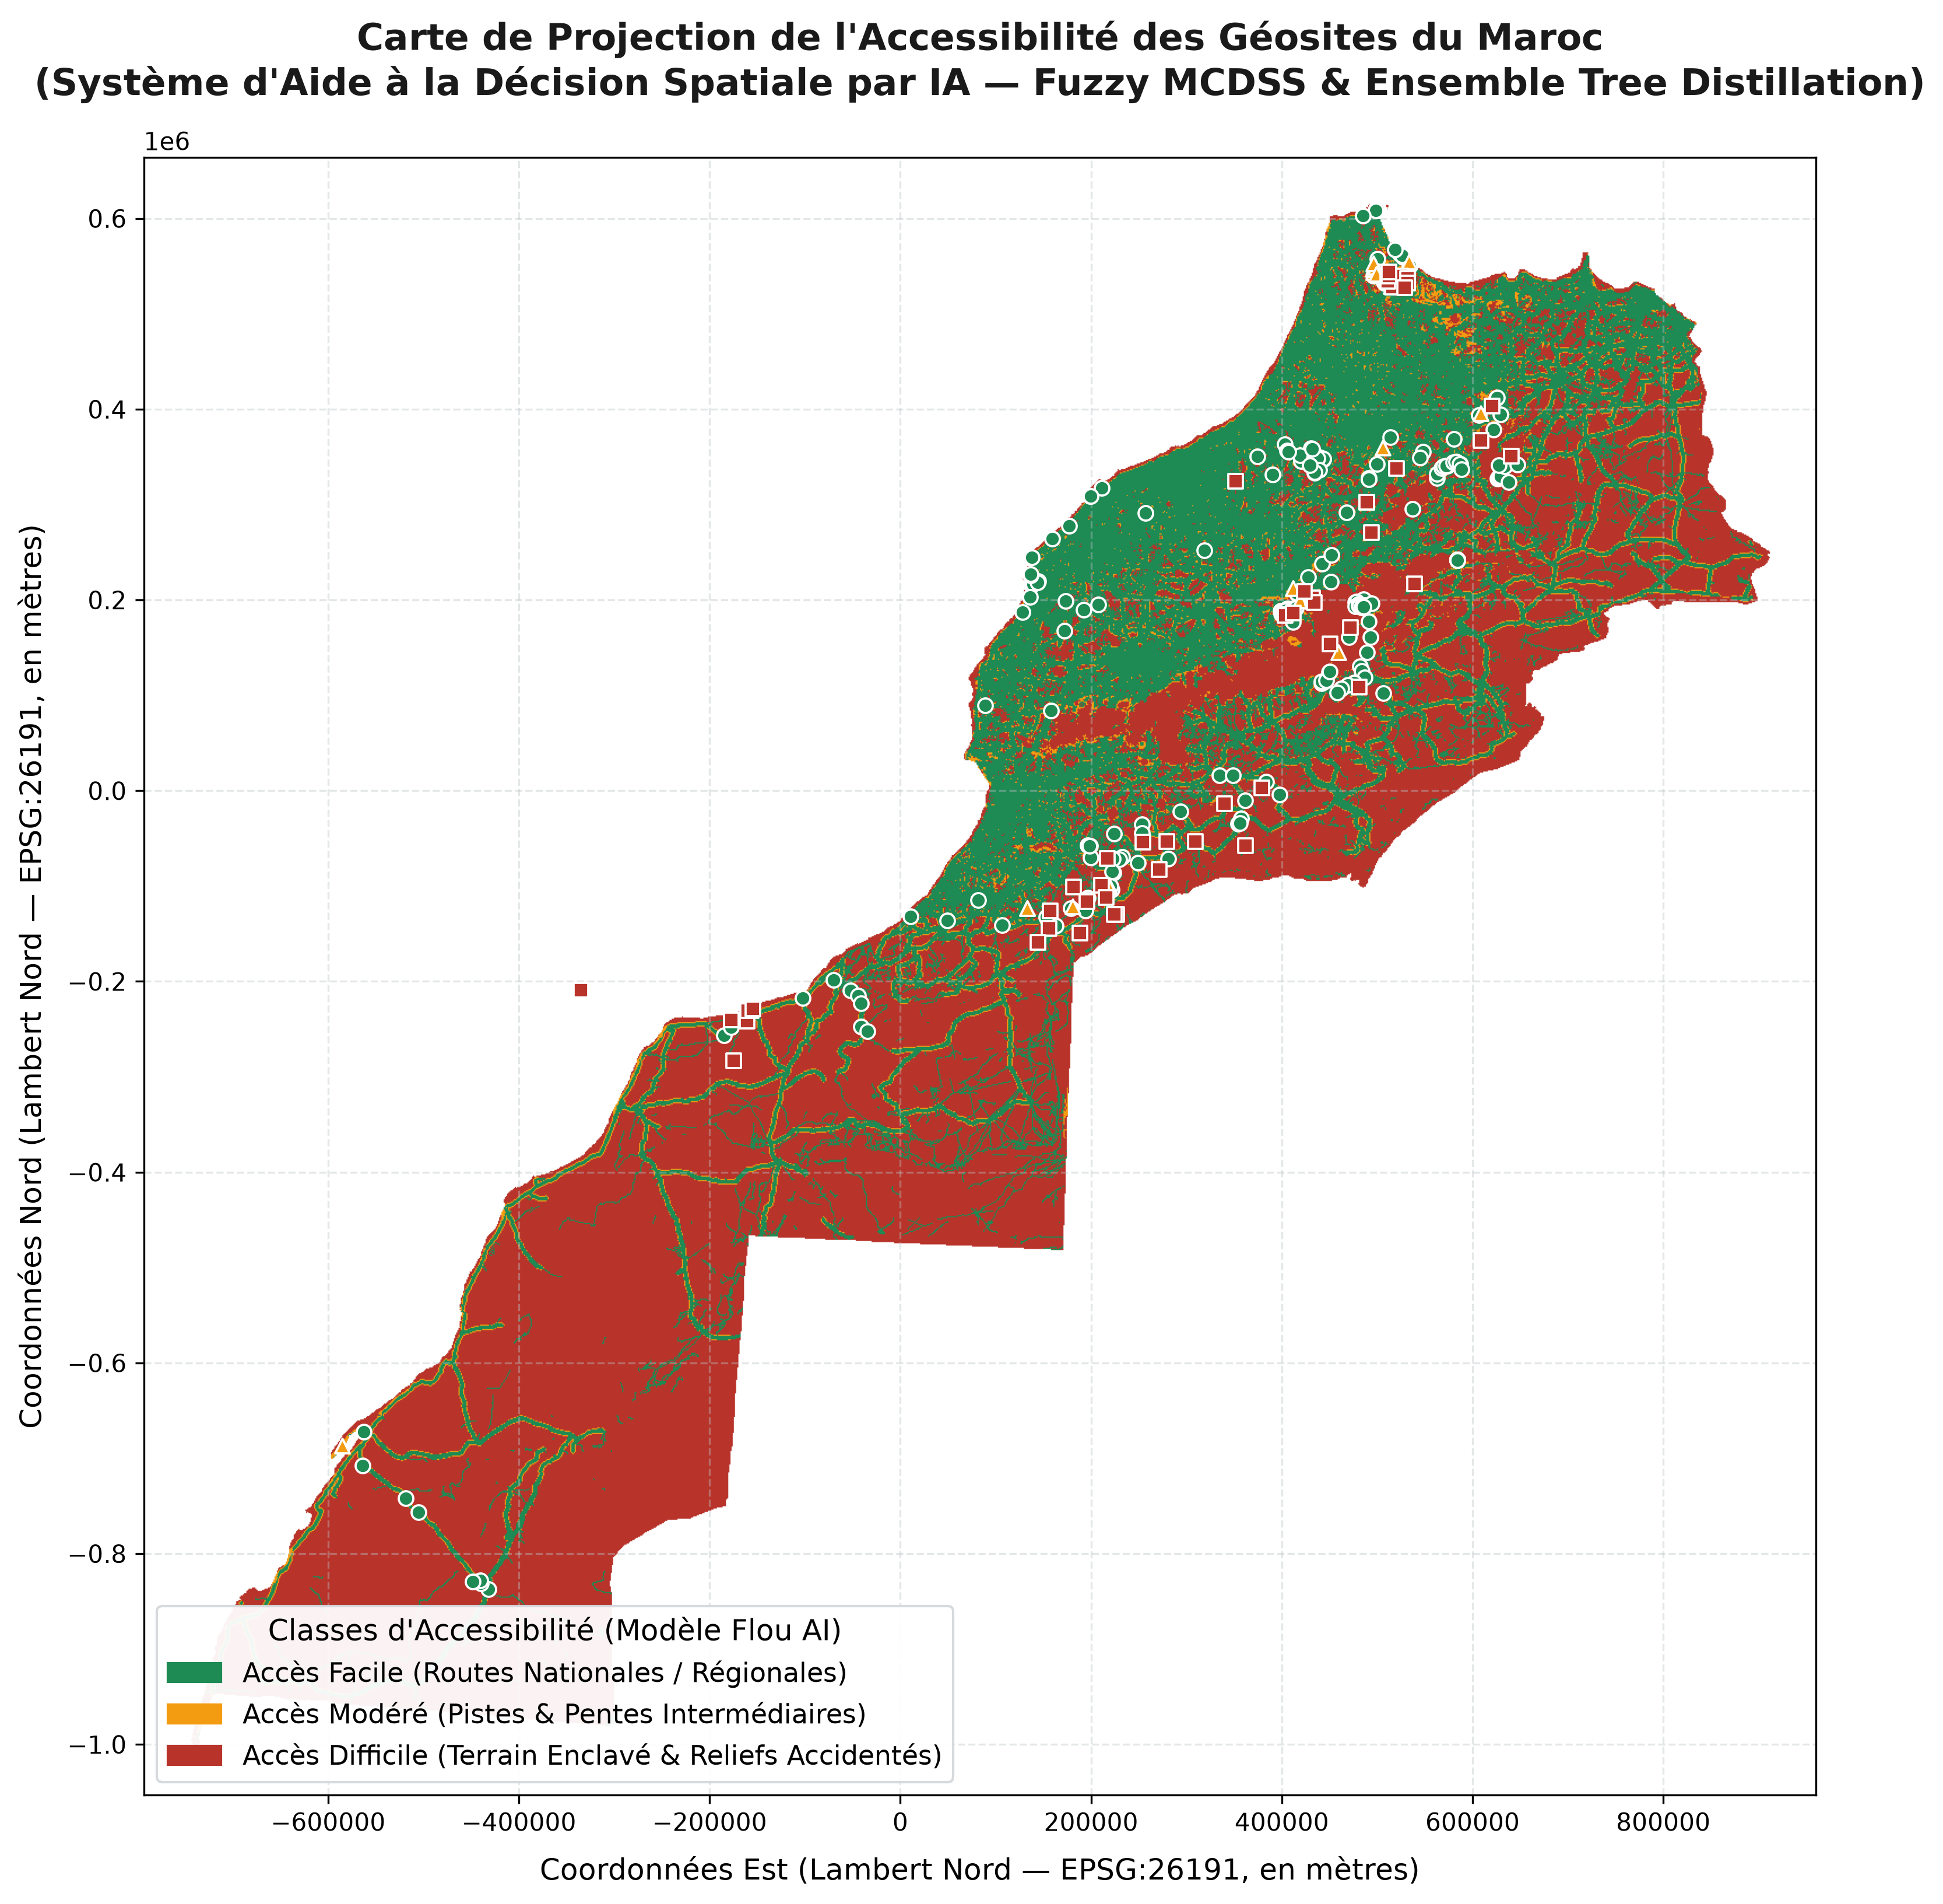
\includegraphics[width=0.9\textwidth]{../figures/morocco_fuzzy_mcdss_accessibility_map.png}
    \caption{Carte projetée de l'accessibilité nationale des géosites du Maroc, montrant la répartition des classes prédites par le modèle Fuzzy MCDSS.}
    \label{fig:map}
\end{figure*}

\section{Conclusions}
En tant que stagiaire de recherche en IA au GSMI-UM6P, j'ai (EL GORRIM Mohamed) mis en place un pipeline scientifique complet et de bout en bout qui permet d'étendre la modélisation des géosites à l'échelle nationale sous une approche floue sans artéfacts de bordure. En introduisant la validation croisée par blocs spatiaux et les fonctions d'appartenance sigmoïdales, nous avons résolu les erreurs de fuite spatiale et de pénalisation artificielle des plaines. Les bases de données, modèles sauvegardés et cartes générés constituent un outil précieux pour le développement régional, la promotion du géotourisme et la conservation du patrimoine géologique national.

\section*{Remerciements}
Nous remercions le Geology and Sustainable Mining Institute (GSMI) et l'Université Mohammed VI Polytechnique (UM6P) pour avoir fourni les ressources et les jeux de données nécessaires à la réalisation de ce projet.

\begin{thebibliography}{1}
\bibitem{naimi2025}
M. Manaouch, L. Naimi, M. Haynou, M. Aghad, M. Sadiki, Q. B. Pham et A. Jakimi, ``Enhancing Geotourism in Southeastern Morocco through Machine Learning-Based Geomorphosite Identification,'' \emph{Geoheritage}, vol. 17, n\textsuperscript{o} 34, 2025.
\end{thebibliography}

\end{document}
